\documentclass[acmsmall]{acmart}

\usepackage{alltt}

\AtBeginDocument{%
  \providecommand\BibTeX{{%
    \normalfont B\kern-0.5em{\scshape i\kern-0.25em b}\kern-0.8em\TeX}}}

\setcopyright{acmcopyright}
\copyrightyear{2020}
\acmYear{2020}
\acmDOI{}

\acmJournal{PACMPL}
\acmVolume{4}
\acmNumber{ICFP}
\acmArticle{42}
\acmMonth{8}

\citestyle{acmauthoryear}

\begin{document}

\title{Harmony and Counterpoint with Dependent Types (Experience Report)}

\author{John Leo}
\affiliation{
  \institution{Halfaya Research}
  \city{Bellevue}
  \state{WA}
  \country{USA}}
\email{leo@halfaya.org}

\author{Youyou Cong}
\affiliation{
  \institution{Tokyo Institute of Technology}
  \city{Tokyo}
  \country{Japan}}
\email{cong@c.titech.ac.jp}

\renewcommand{\shortauthors}{Leo and Cong}

\begin{abstract}

\documentclass[sigplan,screen]{acmart}
\settopmatter{printccs=false, printacmref=false}

\setcopyright{none}
\acmPrice{}
\acmDOI{}
\acmYear{}
\copyrightyear{}
\acmISBN{}
\acmConference[FARM '22]{Proceedings of the 10th ACM SIGPLAN International Workshop on Functional Art, Music, Modeling, and Design}{September 15, 2022}{Ljubljana, Slovenia}
\acmBooktitle{}

%% Bibliography style
\bibliographystyle{ACM-Reference-Format}
%% Citation style
%% Note: author/year citations are required for papers published as an
%% issue of PACMPL.
\citestyle{acmauthoryear}   %% For author/year citations

%% Some recommended packages.
\usepackage{booktabs}   %% For formal tables:
                        %% http://ctan.org/pkg/booktabs
\usepackage{subcaption} %% For complex figures with subfigures/subcaptions
                        %% http://ctan.org/pkg/subcaption
\usepackage{alltt}

\begin{document}

%% Title information
\title{Demo: Counterpoint Analysis and Synthesis}
%\subtitle{Functional Pearl}

%% Author information
%% Contents and number of authors suppressed with 'anonymous'.

\author{John Leo}
\affiliation{
  \institution{Halfaya Research}
  \city{Bellevue}
  \state{WA}
  \country{USA}
}
\email{leo@halfaya.org}


%% Abstract
%% Note: \begin{abstract}...\end{abstract} environment must come
%% before \maketitle command
\begin{abstract}
We present an Agda library to help analyze
and synthesize musical counterpoint. The tool allows expression of
generic constraints in a higher-level musical language which are
translated to a lower level for use both to find rule violations in
existing music and to generate (using an SMT solver) new
music satisfying the constraints. The tool is intended for use by
musicians who need only have a basic knowledge of Agda.
\end{abstract}


%% 2012 ACM Computing Classification System (CSS) concepts
%% Generate at 'http://dl.acm.org/ccs/ccs.cfm'.
\begin{CCSXML}
<ccs2012>
<concept>
<concept_id>10010405.10010469.10010475</concept_id>
<concept_desc>Applied computing~Sound and music computing</concept_desc>
<concept_significance>500</concept_significance>
</concept>
<concept>
<concept_id>10011007.10011006.10011008.10011009.10011012</concept_id>
<concept_desc>Software and its engineering~Functional languages</concept_desc>
<concept_significance>500</concept_significance>
</concept>
</ccs2012>
\end{CCSXML}

\ccsdesc[500]{Applied computing~Sound and music computing}
\ccsdesc[500]{Software and its engineering~Functional languages}
%% End of generated code

%% Keywords
%% comma separated list
\keywords{Counterpoint, Agda, SMT}  %% \keywords are mandatory in final camera-ready submission


%% \maketitle
%% Note: \maketitle command must come after title commands, author
%% commands, abstract environment, Computing Classification System
%% environment and commands, and keywords command.
\maketitle

\section{Introduction}

We demonstrate work in progress on a tool to assist in the analysis and
synthesis of musical counterpoint. Since the mid-18th century, the
composition of counterpoint has been guided by principles enunciated
in Fux's \textit{Gradus ad Parnassum} \citep{Fux1965}, first published
in 1725. Fux presents an increasingly sophisticated series of
``species'' (one note against one note, two notes against one note,
etc.) along with rules governing intervals between notes and motion
between intervals designed to ensure consonance and independence of
voices. It is well documented \citep{Mann1987} that composers
including Haydn, Mozart and Beethoven both studied and taught from
this text, and its fundamentals continue to be taught to music students
today (for example \cite{Kennan1999, Aldwell2018}).

In previous work, Cong and Leo \citep{CongLeo2019} encode the rules of
first-species (note against note) counterpoint as type constructors in
the dependently-typed language Agda. This enforces
correct-by-construction counterpoint and allows use of the Agda
typechecker to return errors with no additional effort required. On
the down side, these errors can be difficult to interpret for those
less familiar with type errors. Furthermore, encoding rules into
constructors is awkward for handling more complex species and more
global constraints. One could separate the construction of the pure
music from the constraints which can be added as a local or global
predicate (as in refinement types), but one may also wish to
deliberately violate some of the rules of strict counterpoint, as
composers often do in practice, and simply be informed of where the
violations occur without being prohibited from incorporating them.

Another approach then is to write a special-purpose ``type checker''
which can be run on previously-created music and which can generate
clear and precise error messages which are musically meaningful. The
checker is ideally easily customizable in terms of what constraints
one would like to impose. It turns out these constraints can be
expressed (at a low level) in the quantifier-free logic of linear
arithmetic and uninterpreted functions (QF-UFLIA \cite{Barrett2010}),
which allows one to not only analyze existing counterpoint, but also
synthesize counterpoint satisfying the constraints using an SMT
(Satisfiablity Modulo Theories) solver.

The initial prototype \citep{HaskellCounterpoint} of this tool was
written in Haskell, chosen due to the availability of the
high-quality and feature-rich SMT library SBV \citep{SBV}. It was then
ported to the Agda Music Tools library \cite{MusicTools}, using Agda's
Haskell foreign function interface (FFI) to call SBV. There is also an
Agda interface \citep{Schmitty} to SMT and we might convert to using
that at some point in the future.

The following sections give an overview of current
functionality. 

\section{An Example}

We briefly describe one way in which this tool can be used for both
analysis and synthesis. We first examine the example numbered 146 in
the critical edition of Beethoven's studies with Haydn
(\cite{BeethovenWerke13}; see also \cite{Nottebohm1971}, p.\ 31 and
\cite{Mann1987}, p.\ 115). It is shown in modern notation in
Figure~\ref{fig:b146}.

\begin{figure}
  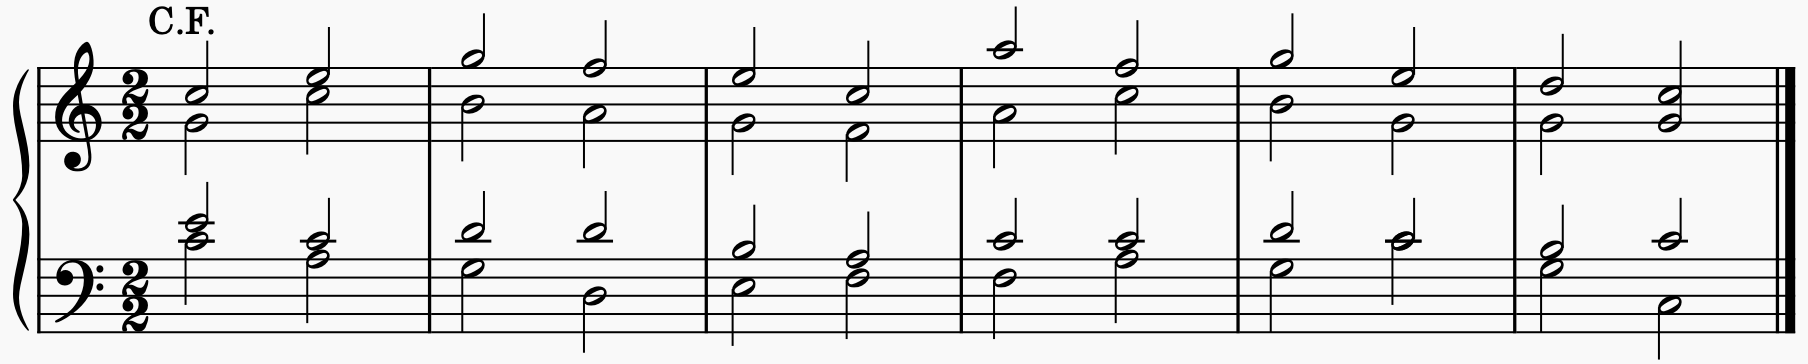
\includegraphics[width=8cm]{figures/b146.png}
  \caption{Beethoven Exercise 146}
  \Description{Beethoven Exercise 146}
  \label{fig:b146}
\end{figure}

Here Haydn has supplied the top voice, marked ``C.F.'' for cantus
firmus, and Beethoven's task was to supply the remaining three voices
following first species counterpoint rules. He uses only tones from
triads, all of them complete save the last and all in root position
save the second triad in bar 4. Since the notes form triads they
automatically satisfy consonance rules (only perfect intervals, thirds
or sixths between any pair of notes vertically); note that a perfect
fourth is prohibited in two part strict counterpoint but allowed with
more voices. Perfect fourths can be found between the top two voices
in the first, fourth and last bars.

There are boundary rules that the top and bottom voices must form
octaves at the beginning and end, and motion rules which are designed
to ensure independence of voices. In particular parallel and similar
(both voices moving in the same direction) motion into fifths and
octaves is prohibited. Here we can see that Beethoven has in fact made
two errors in the top two voices: similar motion into a fifth in bar 3
and then into an octave between bars 3 and 4. Haydn fixes both errors
by changing the F in the second voice (marked with the red X) to an A.

For simplicity we now focus only on the top two voices. Feeding
Beethoven's notes into the tool as two part first species
counterpoint, it easily finds and reports errors in the use of perfect
fourths, missing octaves at the boundaries, and similar motion into
fifths and octaves. We can disable the boundary rules as they are not
relevant and relax the consonance rule to allow perfect fourths, leaving
only the motion errors. We can replace the note F that Haydn fixed
with a hole, and run the tool in synthesis mode using the same
rules. It makes the same fix Haydn did. Perhaps we gave it too much
guidance, so instead we can create three holes in a row near the
error, which generates the solution shown in
Figure~\ref{fig:b146fix3}. Note that this introduces a series of five
parallel 6ths, and there is a ``soft'' rule that one should not have
long sequences of 3rds or 6ths as that also diminishes independence
of voices. However we can easily add a constraint limiting parallel
intervals to at most two in a row; the solution returned changes the G
in bar three to an A, breaking the chain with a fifth, a small
improvement but one might hope for more.

\begin{figure}
  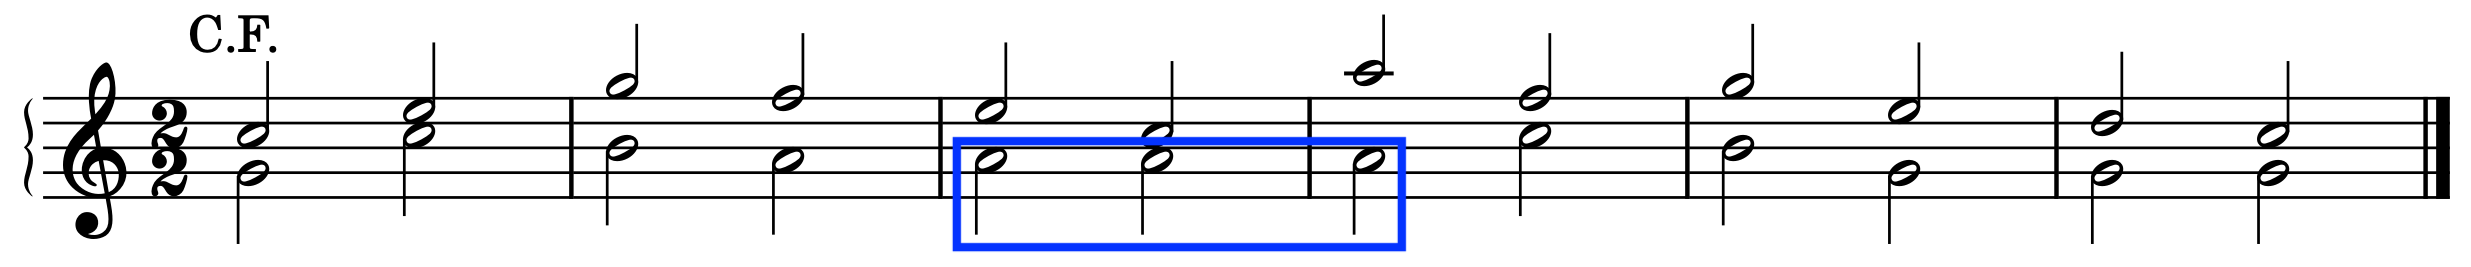
\includegraphics[width=8cm]{figures/b146fix3.png}
  \caption{Three Notes Changed}
  \Description{Three Notes Changed}
  \label{fig:b146fix3}
\end{figure}

This can be done by adding a constraint to increase contrary motion
(in which both voices move in opposite directions), and in fact we can
try generating our own two part counterpoint following Haydn's cantus
firmus, fixing only the first and last of Beethoven's notes. To help
create better quality counterpoint we add constraints to limit the
number of leaps (horizontal intervals of more than a major third) to
at most one and require at least six instances of contrary motion,
which turns out to be maximal. Note that it would be extremely
difficult for a human being with no computer assistance to generate
counterpoint following such restrictions, but the SMT solver instantly
returns the solution shown in Figure~\ref{fig:b146gen3}.

\begin{figure}
  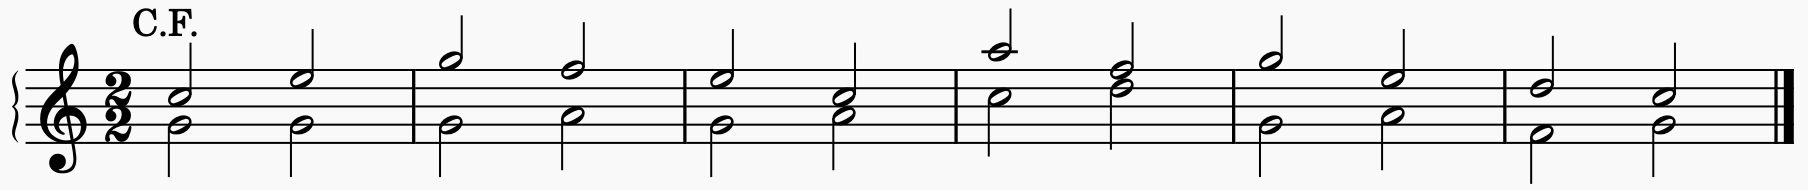
\includegraphics[width=8cm]{figures/b146gen3.png}
  \caption{Generated Counterpoint}
  \Description{Generated Counterpoint}
  \label{fig:b146gen3}
\end{figure}


\section{Selected Features}

We describe at a high level some of the key features of the
library. Details can be found in the code repository
\citep{HaskellCounterpoint}.

At a high level music is represented as a list of voices, which in
turn are a list of bars, which are in turn a list of beats. Here
dependent types would be useful to ensure for example that every voice
has the same number of bars, but a run-time check can also be used to
enforce this. Each of these elements is parameterized, allowing a
number of pitch-like elements to be used to construct music. These
could be algebraic data types representing name (like G\#) and
octave, or a numeric representation of pitch. Either datum can then be
embedded into a wrapper, such as \texttt{MPitch} which can either be a
fixed pitch or a named hole to be solved for.

The above representation of music allows natural handling of first,
second and third species counterpoint (one to four notes per cantus
firmus note) as well as multi-part counterpoint. At a lower level the
music is translated into a simpler form---for example first-species
two part counterpoint is most simply represented as a list of pairs.

We plan to try to implement a constraint language as an embedded
DSL. However for now Haskell typeclasses are used, which have the
advantage that constraints can be written in natural Haskell; the only
drawback is that type signatures are somewhat abstract. The main
challenge is that we want to write constraints only once and use them
for both analysis and synthesis. The former expects low-level integers
and booleans while the latter their symbolic counterparts. This is
handled by using typeclasses which can be instantiated with either.

Analysis and synthesis then both take the same music and list of
constraints. The former checks the constraints returning error
messages in the higher-level language used to express the music. The
latter generates (if possible) music by filling in the given holes
using the constraints and the SMT solver. MIDI is also generated,
which can then be opened and viewed with notation software such as
MuseScore.

\section{Future Plans}

Future plans include possible integration with Liquid Haskell
\citep{LiquidHaskell} (for analysis) and Synquid \citep{Synquid} (for
synthesis). In addition to handling higher species we would like to
also incorporate the rules and conventions of galant schemata
\citep{Gjerdingen2007}, which informed much of the music composed in
the era of Haydn and Mozart. Ideally one could use the tool to compose
convincing music in the galant style.

Concurrently Cong \citep{Cong2022a,Cong2022c} is exploring another approach
using a different representation of constraints within a type system.
Recent work by Tanaka \citep{Tanaka2022} uses integer programming to
express constraints, and we plan to compare our method with this.

\section*{Acknowledgements}

Thanks to Youyou Cong for many enlightening discussions about type
theory and music over the past several years, and for suggesting to
look at Beethoven's exercises as a source of examples. Thanks also to
Emina Torlak and Stephen Rumph for their generosity in allowing me to
audit their classes at the University of Washington. CSE 507 was
invaluable for learning the fundamentals of SMT 
solvers, and MUHST 211 and 430 introduced me to galant schemata.
Finally, thanks the anonymous referees for many helpful comments and
suggestions.

%% Bibliography
\bibliography{abstract.bib}

\end{document}


\end{abstract}

\keywords{dependent types, harmony, counterpoint}

\maketitle

\section{Introduction}
\label{sec:intro}

Edgar Var\`{e}se describes music as ``organized sound'', and
throughout history cultures have developed and applied systems of rules
and guidelines to govern the music they create, most notably the
Common Practice Period of Western music spanning the 17th to early
20th centuries. These rule systems are seldom absolute, and indeed
deliberate breaking of the rules is often part of the aesthetic, but they
roughly constrain the music they apply to and
give it a common form and sound.

Artists and theoreticians have attempted to capture and codify these
rule systems, informally in natural language, and typically
accompanied by examples from the existing literature. The intent is
both to analyze existing music and then to use these principles to
guide the creation of new music, in other words for synthesis.

Starting in the 20th century, computers have become ubiquitous in
music in every area, including sound synthesis, composition and
production~\citep{roads-tutorial}. In terms of music theory, there has
been a line of recent work on using functional programming for
harmonic
analysis~\citep{magalhaes-harmtrace,dehaas-harmtrace-a,dehaas-harmtrace-b},
harmonization of a melody and generation of melodies based on a
harmonization~\citep{koops-fharm,magalhaes-fcomp} and
counterpoint~\citep{szamozvancev-welltyped}. There is also an
established Haskell library Euterpea~\citep{hudak-haskell} for general music
and sound exploration.

To describe rules of basic harmonic structure,
\citet{magalhaes-harmtrace} and their successors use dependent types,
for example to index chords by major or minor mode.  However Haskell
currently has limited support for dependent types, and requires many
extentions and tricks such as the use of singleton
types~\citep{eisenberg-singleton}.

In this paper we explore what can be done in the context of music by
using a programming language that offers full dependent types. We use
Agda~\citep{norell-phd} since it is fairly mature and
aims to be both a functional programming language and a proof
assistant. It also features a Haskell FFI so we can take advantage of
existing Haskell libraries, in particular for MIDI generation.

% However this is difficult because most
% ``rules'' in music theory are not absolute, but rather suggestions of
% varying degrees (themselves vaguely specified) of importance. Since
% ultimately the resulting created music is more important than the
% theory, an alternative is to attempt to indirectly deduce the rules
% from music samples, using machine learning~\citep{huang-cp} or
% some other statistical methods. Unfortunately the set of deduced
% rules could sometimes be insufficient for generating good music.
% As an example, \citet{roberts-cp} develop the Bach Doodle
% harmonization tool using Bach chorals as training data, but still
% observe high frequency of parallel 5th and 8th that are extremely
% rare in Bach's music.

% Ultimately it seems some kind of mixture of rules and statistics may
% be the best way to faithfully capture an effective theory of
% music. One simple approach would be to develop a logic of rules and
% their interactions, but attach weights to the rules which could be
% determined via machine learning techniques.

Full dependent types allow expression of predicate logic, and it is
tempting to take a standard textbook on music theory such as
\citet{piston-harmony} or \citet{aldwell2018harmony} and formalize it
in type theory.  As a first step towards this goal, we start with the modest task of
expressing a small, relatively strict rule set known as species
counterpoint~\cite{fux-cp}, intended for combining interdependent
melody lines to produce a pleasant-sounding result.  Roughly speaking,
what we do is to write a custom musical type checker in Agda.
Compared to the previous work by \citet{cong-cp}, where rules are
expressed directly as Agda types, our approach makes it easier to
describe fine-grained rules, produce readable error messages, and add
or drop rules depending on the circumstances.

% [NOTE: I've squeezed the description of our new counterpoint
% implementation.]

% We make use of and extend Music Tools~\citep{MusicTools},
% a library of small tools
% for analysis and synthesis of music written in Agda, with the goal of
% eventually being a dependently-typed alternative to Euterpea.
% Previous work by \citet{cong-cp} expresses
% first-species counterpoint with the Agda type system, so that an error
% in counterpoint results in an Agda type error. Although this takes
% advantage of Agda's native type checking, it has several
% downsides. One is that the Agda errors may be difficult to interpret
% as the corresponding musical error. Another is that it is difficult to
% keep the types both simple and flexible.

% In this work we present an alternative representation of counterpoint
% using what could be considered a custom musical type checker written
% in Agda. This allows us to easily describe fine-grained rules, write
% custom type errors, and then combine subsets of rules together for
% larger-scale checking. Music can be combined with rules it
% satisfies as a dependent record type. This record represents a proof
% certificate that the music follows the asserted rules.
% Rules can also be used in multiple different contexts, satisfying
% modularity and composability.

We also present preliminary work on harmonizing a melody using
a subset of rules based on \citet{piston-harmony}, contrasting with
existing work by \citet{koops-fharm}. Since counterpoint and
harmony are not separate concepts but in fact deeply intertwined, we
would wish to reuse counterpoint rules to develop natural-sounding
harmonizations.  We show that, with our custom type checker, it is
straightforward to reuse rules in different contexts.  Put differently,
our representation of rules satisfies modularity.

The rest of this paper structured as follows.  Section~\ref{sec:music}
introduces basic musical concepts as well as their Agda representation.
Sections~\ref{sec:cp} and \ref{sec:harmony} describe our formalization
of counterpoint and harmony, focusing on the composable and
modular aspects of the proposed approach.  Lastly,
Section~\ref{sec:conclusion} concludes the paper with future perspectives.

This is an experience report, and we highlight both the advantages and
disadvantages of using Agda for music theory. On one hand the
expressiveness of dependent types makes it easy and natural to
describe music theory rules. On the other hand we find the emphasis on proof
construction and particularly the extra work needed for decidable
equality can add an extra burden which is not always welcome. However
overall we feel the positives far outweigh the negatives, and in the
final section we discuss possible ways to reduce the tedium.

Our implementation is available as the anonymized supplement.
\section{Musical Preliminaries}
\label{sec:music}

\paragraph{Pitches}
In music, a \emph{pitch} is a value denoting how high or low a sound is.
Pitches can be represented either as an absolute value or as a relative
value paired with the octave the sound belongs to.
In our implementation, the two representations of pitches are defined
as \texttt{Pitch} and \texttt{PitchOctave}, respectively, accompagnied
by a proof that converting back and forth between them is an identity.

\begin{alltt}
data Pitch : Set where
  pitch : \(\mathbb{N}\) \(\rightarrow\) Pitch

data Octave : Set where
  octave : \(\mathbb{N}\) \(\rightarrow\) Octave

PitchOctave : Set
PitchOctave = Fin 12 \(\times\) Octave
\end{alltt}

\paragraph{Duration}
\emph{Duration} denotes a certain unit of time during which a sound
or silence lasts.
The unit is unspecified at the composition time; it is instantiated to
a concrete value when the music is played at a specific tempo.

\begin{alltt}
data Duration : Set where
  duration : \(\mathbb{N}\) \(\rightarrow\) Duration
\end{alltt}

\paragraph{Note}
Combining pitches and duration gives us \emph{notes}.
In our implementation, we represent notes with sound as \texttt{tone}s
and those without as \texttt{rest}s.

\begin{alltt}
data Note : Set where
  tone : Duration \(\rightarrow\) Pitch \(\rightarrow\) Note
  rest : Duration         \(\rightarrow\) Note
\end{alltt}

\paragraph{Intervals}

\emph{Intervals} are yet another key concept in music.
An interval denotes the difference in pitch between two notes.
There are 13 kinds of interval within an octave, and these intervals
may be classified from several different perspectives: (i) major or minor;
(ii) consonant or dissonant; and (iii) perfect or imperfect.
For convenience, we let the names of intervals carry the information
about the first and third classifications.
As a convention, we refer to \texttt{min2} and \texttt{maj2}  uniformly
as ``2nd'', and similarly for other intervals.
We also call \texttt{per1} the \emph{unison} in the rest of this section.

\begin{figure}[h]
  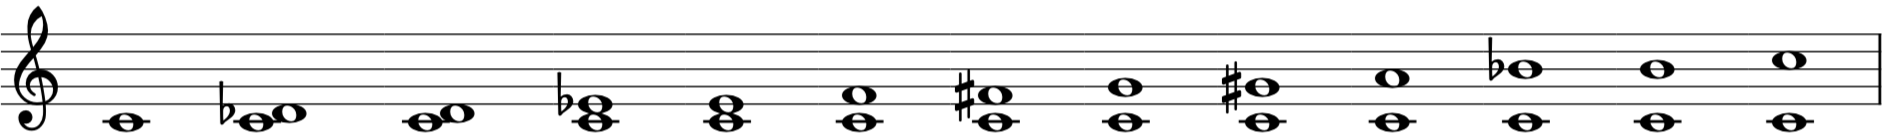
\includegraphics[width=12cm]{interval.png} \\
  \begin{flushleft}
    \begin{small}
      \hspace{1.45cm} per1 \ \ \ min2 \ \ \ \ maj2 \ \ \ min3 \ \ maj3
      \ \ per4 \ \ aug4 \ \ \,per5 \ \ min6 \ \,maj6 \ \,min7 \ \,maj7 \ \,per8
    \end{small}
  \end{flushleft}
\end{figure}
  
\begin{alltt}
data Interval : Set where
interval : \(\mathbb{N}\) \(\rightarrow\) Interval

per1  = interval 0 -- consonant
min2  = interval 1
maj2  = interval 2
min3  = interval 3 -- consonant
maj3  = interval 4 -- consonant
per4  = interval 5 
aug4  = interval 6
per5  = interval 7 -- consonant
min6  = interval 8 -- consonant
maj6  = interval 9 -- consonant
min7  = interval 10
maj7  = interval 11
per8  = interval 12 -- consonant
\end{alltt}

\newcommand{\FS}{
  \begin{figure}
    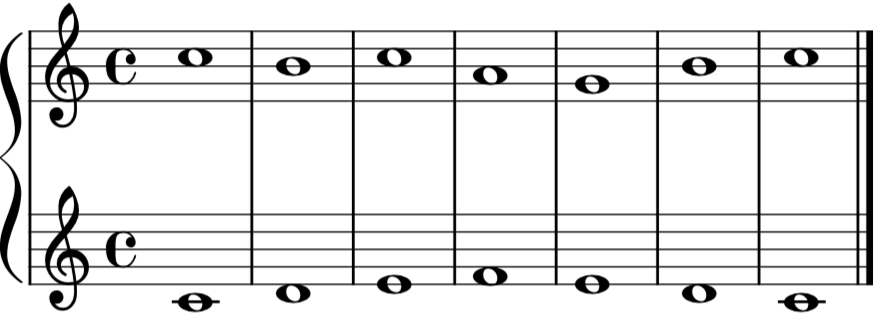
\includegraphics[width=6cm]{fig/fs.png}
    \caption{First Species Counterpoint}
    \label{fig:fs}
  \end{figure}
}

\newcommand{\Motion}{
  \begin{figure}
    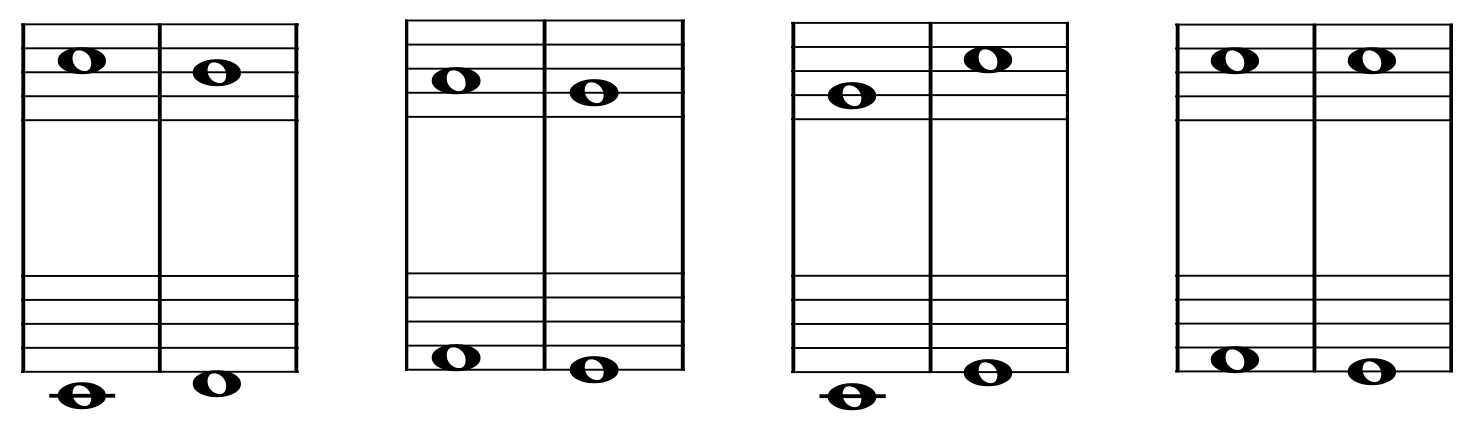
\includegraphics[width=11cm]{fig/motion.png}
    \begin{flushleft}
    \begin{small}
      \hspace{1.65cm} contrary \ \ \ \ \ \ \ parallel \ \ \ \ \ \ \ \
      \ \ similar \ \ \ \ \ \ \ \ \ oblique
      \hspace{1cm} paralell-5th \ \ \ similar-8th
    \end{small}
    \end{flushleft}
    \caption{Four Kinds of Motion (left) and Invalid Patterns (right)}
    \label{fig:motion}
  \end{figure}
}

\renewcommand{\SS}{
  \begin{figure}
    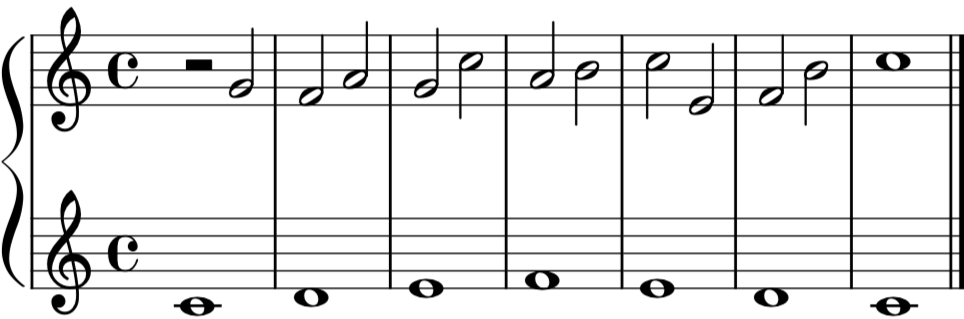
\includegraphics[width=7cm]{fig/ss.png}
    \caption{Second Species Counterpoint}
    \label{fig:ss}
  \end{figure}
}

\section{Counterpoint}
\label{sec:cp}

TODO: contrast old and new methods

Counterpoint is a technique for combining multiple lines of melodies.
Composing counterpoint is like arranging a song for choir:
we start with a \emph{cantus firmus}, which serves as the base melody,
and compose counterpoint lines above or below the cantus firmus.
When doing this, we must make sure that the whole music sounds
harmonically pleasing, and that the individual melodic lines are
distinguishable to the listener.

In this section, we present an implementation of species counterpoint,
based on the formulation given by Fux~\citep{fux-cp}.
The idea is to represent ``good'' counterpoint  as a dependent record,
whose fields encode the musical content as well as proofs that the
counterpoint follows certain rules.
For space reason, we only describe two variants of species counterpoint;
other variants can be formalized in an analogous way.

\subsection{First Species Counterpoint}
\label{sec:cp:fs}

\FS

First species counterpoint is the simplest variant of counterpoint.
In first species, we set one note against each note in the cantus firmus,
which is required to start with a tonic and consist only of whole notes.
Figure~\ref{fig:fs} shows an example of first species counterpoint.
The lower line is the cantus firmus, which we excerpt from a famous
German song called ``Froschgesang'' (Frog's song).
The upper line is the counterpoint composed by the second author.

\subsubsection{Representing Music}

In our implementation, we represent each bar as a pitch-interval pair
\texttt{(p ,  i)}, where \texttt{p} is the pitch of a cantus firmus note,
and \texttt{i} is the interval between \texttt{p} and the corresponding
counterpoint note.
We then represent a sequence of bars as a list of pitch-interval pairs,
but with one proviso: we separate the first and last bars from the
middle bars.
Therefore, the Frog's song in Figure~\ref{fig:fs} is represented as a
compound of the following three elements:

\begin{alltt}
 PitchInterval : Set
 PitchInterval = Pitch \(\times\) Interval
  
first : PitchInterval
first = (c 5 , per8)

middle : List PitchInterval
middle = (d 5 , maj6) :: (e 5 , min6) :: (f 5 , maj3) ::
         (e 5 , min3) :: (d 5 , maj6) :: []

last : PitchInterval
last = (c 5 , per8)
\end{alltt}

\subsubsection{Representing Rules}

The reason behind our three-part representation of music is that
different parts are subject to different rules, as we detail below.

\paragraph{Beginning}

The beginning of the music should express perfection.
As we saw in Section~\ref{sec:music}, there are three intervals that
are classified as perfect: the 1st (more commonly called the
\emph{unison}), the 5th, and the 8th.
The first interval of the music must then be one of these intervals.
In our formalization, we implement this rule as the
\texttt{checkBeginning} function, which reports an error
\texttt{not158 i} when the first interval \texttt{i} is an invalid one.
Since Agda does not have exceptions, we turn the error into an option
value by wrapping it around the \texttt{just} constructor.

\begin{alltt}
data BeginningError : Set where
  not158   : PitchInterval \(\rightarrow\) BeginningError
  
checkBeginning : PitchInterval \(\rightarrow\) Maybe BeginningError
checkBeginning pi@(_ , i) =
  if ((i == per1) \(\vee\) (i == per5) \(\vee\) (i == per8))
  then nothing
  else just (not158 pi)
\end{alltt}

\paragraph{Intervals}

The middle bars of the music should maintain harmonical consonance
and independence of melodic lines.
As we saw before, consonant intervals include the unison,
3rd\footnote{We use ``3rd'' to mean both the major and minor variants
of the 3rd interval, and similarly for the 6th.}, 5th, 6th, and 8th,
and among these, the unison is clearly an obstacle to distinguishing
between the two lines of music.
Therefore, the middle bars must consist of the latter four intervals.
We encode this rule as the \texttt{checkIntervals} function, which
returns a list of errors correponding to the occurrences of dissonant
intervals and unisons.

\begin{alltt}
data IntervalError : Set where
  dissonant : Interval \(\rightarrow\) IntervalError
  unison    : Pitch \(\rightarrow\) IntervalError

intervalCheck : PitchInterval \(\rightarrow\) Maybe IntervalError
intervalCheck (p , i) with isConsonant i | isUnison i
... | false | _    = just (dissonant i)
... | _     | true = just (unison p)
... | _     | _    = nothing

checkIntervals : List PitchInterval \(\rightarrow\) List IntervalError
checkIntervals = mapMaybe intervalCheck
\end{alltt}

\paragraph{Motion}

\Motion

The independence of melodic lines is also affected by \emph{motion},
i.e., the way one interval moves to another interval.
As can be seen from Figure~\ref{fig:motion} left, there are four
kinds of motion: \emph{contrary} (two lines go in different directions),
\emph{parallel} (two lines go in the same direction by the same
distance), \emph{similar} (two lines go in the same direction),
and \emph{oblique} (one line plays the same note).
There is a consensus that approaching a perfect interval by parallel
or similar motion (as in Figure~\ref{fig:motion} right) destroys the
independence of lines.
To rule out this, we define the \texttt{checkMotion} function, which
lists all occurrences of such invalid motion.

\begin{alltt}
data MotionError : Set where
  parallel : PitchInterval \(\rightarrow\) PitchInterval \(\rightarrow\) MotionError
  similar  : PitchInterval \(\rightarrow\) PitchInterval \(\rightarrow\) MotionError

motionCheck : PitchInterval \(\rightarrow\) PitchInterval \(\rightarrow\) Maybe MotionError
motionCheck i1 i2 with motion i1 i2 | isPerfect (proj\(\sb{\mathtt{2}}\) i2)
motionCheck i1 i2 | contrary | \_     = nothing
motionCheck i1 i2 | oblique  | \_     = nothing
motionCheck i1 i2 | parallel | false = nothing
motionCheck i1 i2 | parallel | true  = just (parallel i1 i2)
motionCheck i1 i2 | similar  | false = nothing
motionCheck i1 i2 | similar  | true  = just (similar i1 i2)

checkMotion : List PitchInterval \(\rightarrow\) List MotionError
checkMotion = mapMaybe (uncurry motionCheck) \(\circ\) pairs
-- where pairs returns a list of all adjacent pairs in a given list
\end{alltt}

\paragraph{Ending}

The ending of the music should express relaxation.
Among different intervals, the unison and the 8th are considered
most stable, hence the last interval of the music must be either of
these intervals.
The last interval should also be approached by a \emph{cadence},
a progression that gives rise to a sense of resolution.
We encode these rules as the \texttt{checkEnding} function.
Note that it returns the \texttt{tooShort} error when the music does
not have enough number of bars to form a valid ending.

\begin{alltt}
data EndingError : Set where
  not18    : PitchInterval \(\rightarrow\) EndingError
  not27    : PitchInterval \(\rightarrow\) EndingError
  tooShort : List PitchInterval \(\rightarrow\) EndingError

endingCheck : PitchInterval \(\rightarrow\) PitchInterval \(\rightarrow\) Maybe EndingError
endingCheck pi1@(pitch p , i) (pitch q , interval 0)  = 
  if ((p + 1 \(\equiv\sp{\mathtt{b}}\) q) \(\wedge\) (i == min3)) then nothing else just (not27 pi1)
endingCheck pi1@(pitch p , i) (pitch q , interval 12) =
  if ((q + 2 \(\equiv\sp{\mathtt{b}}\) p) \(\wedge\) (i == maj6) \(\vee\) (p + 1 \(\equiv\sp{\mathtt{b}}\) q) \(\wedge\) (i == min10))
  then nothing
  else just (not27 pi1)
endingCheck pi1               pi2                     =
  just (not18 pi2)

checkEnding : List PitchInterval \(\rightarrow\) PitchInterval \(\rightarrow\) Maybe EndingError
checkEnding []        \_ = just (tooShort [])
checkEnding (p :: []) q = endingCheck p q
checkEnding (p :: ps) q = checkEnding ps q
\end{alltt}

\subsubsection{Putting Things Together}

Using the encoding of music and rules we have seen so far, we define
\texttt{FirstSpecies}, a record type inhabited by correct counterpoint.
The first three fields of this record type represent the first, middle,
and last bars, respectively.
The last four fields stand for the proofs that the music satisfies all
the required properties, that is:

\begin{itemize}
  \item The beginning is a perfect consonance
  \item The middle bars have no dissonant interval or unison
  \item The middle bars have no perfect interval approached by
    parallel or similar motion
  \item The ending is a unison or an octave approached by a cadence
\end{itemize}

\noindent Recall that the functions representing these rules return
either an option value or a list of found errors.
Therefore, the correctness proofs either take the form
\texttt{func args $\equiv$ nothing}, or look like
\texttt{func args $\equiv$ []}.

\begin{alltt}
record FirstSpecies : Set where
  constructor firstSpecies
  field
    firstBar    : PitchInterval
    middleBars  : List PitchInterval
    lastBar     : PitchInterval
    beginningOk : checkBeginning firstBar \(\equiv\) nothing
    intervalsOk : checkIntervals middleBars \(\equiv\) []
    motionOk    : checkMotion middleBars \(\equiv\) []
    endingOk    : checkEnding middleBars lastBar \(\equiv\) nothing
\end{alltt}

With this record type, we can show that the counterpoint in
Figure~\ref{fig:fs} is correct, since the music is an inhabitant of
the \texttt{FIrstSpecies} type.

\begin{alltt}
fs : FirstSpecies
fs = firstSpecies first1 middle1 last1 refl refl refl refl
\end{alltt}

\subsection{Second Species Counterpoint}
\label{sec:cp:ss}

\SS

We next discuss a more complex variant of counterpoint, called the
second species.
In second species, we set \emph{two} half notes against every cantus
firmus note.
Figure~\ref{fig:ss} is an example of such two-against-one counterpoint,
again composed for the Frog's song.

\subsubsection{Representing Music}

In second species, the first and last bars may have a different structure
from middle bars.
More specifically, it is encouraged to begin the counterpoint line with
a half rest and end with a whole note.
Therefore, in our implementation, we reuse the \texttt{PitchInterval} 
type for the first and last bars, and define a new type
\texttt{PitchInterval2} for middle bars:

\begin{alltt}
PitchInterval2 : Set
PitchInterval2 = Pitch \(\times\) Interval \(\times\) Interval

first2 : PitchInterval
first2 = (c 5 , per5)

middle2 : List PitchInterval2
middle2 =
  (d 5 , min3 , per5) :: (e 5 , min3 , min6) :: (f 5 , maj3 , aug4) ::
  (e 5 , min6 , min3) :: (d 5 , min3 , maj6) :: []

last2 : PitchInterval
last2 = (c 5 , per8)
\end{alltt}

\subsubsection{Representing Rules}

In second species counterpoint, some parts of the music are applied
the same rules as first species, while other parts are constrained by
new rules.

\paragraph{Beginning}

The beginning of the music is \emph{not} allowed to be the unison,
as it prevents the listener from recognizing the beginning of the
counterpoint line.
We restrict the first interval by defining a new error
\texttt{BeginningError2} and a function \texttt{checkBeginning2}
that works analogously to \texttt{checkBeginning} for first species.

\paragraph{Strong Beats}

The rhythmic structure of secound species counterpoint gives rise to
the distinction between \emph{strong beats} (the first interval in a bar)
and \emph{weak beats} (the second interval).
Strong beats in middle bars are constrained by the same rules as in
first species.
That is, they must all be consonant, non-unison intervals, and in the 
case of perfect intervals, the motion from the preceding interval (on
the weak beat) must be either contrary or oblique.
We encode these restrictions as the \texttt{checkStrongBeats}
function, which, as the \texttt{checkIntervals} function for first
species, returns a list of found errors.

\paragraph{Weak Beats}

Compared to strong beasts, weak beats are constrained in a looser
manner.
First, they are allowed to be dissonant if they are created by a
\emph{passing tone}, i.e., a note in the middle of two step-wise
motions in the same direction (as in bars 4-5 of Figure~\ref{fig:ss}).
Second, they are allowed to be the unison if they are left by step in
the opposite direction from their approach (as in bars 5-6 of
Figure~\ref{fig:ss}).
We implement these rules as the \texttt{checkWeakBeats} function,
which checks the validity of every three successive beats in the
middle bars.

\paragraph{Motion}

Parallel and similar motion towards a perfect interval is prohibited
across bars.
We enforce this rule using the \texttt{checkMotion2} function,
which uses \texttt{expandPitchIntervals2} to convert a list of
\texttt{PitchInterval2} into a list of \texttt{PitchInterval}, and
checks every pair of weak beat and strong beat intervals.

\subsubsection{Putting Things Together}

Now we define \texttt{SecondSpecies}, a record type inhabited by
correct second species counterpoint.
As in \texttt{FirstSpecies}, we have three fields holding the musical
content, followed by five fields carrying the proofs of various
properties.

\begin{alltt}
record SecondSpecies : Set where
  constructor secondSpecies
  field
    firstBar      : PitchInterval 
    middleBars    : List PitchInterval2
    lastBar       : PitchInterval 
    beginningOk   : checkBeginning2 firstBar \(\equiv\) nothing
    strongBeatsOk : checkStrongBeats middleBars \(\equiv\) []
    weakBeatsOk   : checkWeakBeats middleBars (secondPitch lastBar) \(\equiv\) []
    motionOk      : checkMotion2 (firstBar ::
                                  (expandPitchIntervals2 middleBars) ++
                                  (lastBar :: [])) \(\equiv\) []
    endingOk      : checkEnding2 middleBars lastBar \(\equiv\) nothing
\end{alltt}

Using \texttt{SecondSpecies}, we can show that the second species
counterpoint in Figure~\ref{fig:ss} is correct.

\begin{alltt}
ss : SecondSpecies
ss = SecondSpecies first2 middle2 last2 refl refl refl refl refl
\end{alltt}

\newcommand{\Harmonization}{
  \begin{figure}
    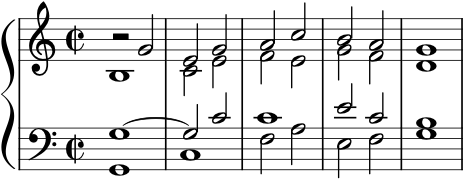
\includegraphics[width=5.5cm]{fig/piston.png}
    \hspace{1cm}
    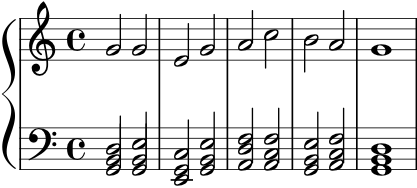
\includegraphics[width=5cm]{fig/fharm.png} \\
    \begin{flushleft}
    \begin{small}
     \hspace{2.35cm} V \ \ \ \ \ \ \ \,I \ \ \ \ \ \ \ \,IV \,VI \ \,III \ IV \ \ \,V
     \hspace{2.6cm} V \ \ \ \ \ \ \ \,I \ \ \ \ \ \,IV VI \,III\,IV \ \ V
    \end{small}
    \end{flushleft}
    \caption{Harmonization by Piston (left) and \fharm (right)}
    \Description{Harmonization by Piston (left) and \fharm (right)}
    \label{fig:harmonization}
  \end{figure}
}

\section{Harmony}
\label{sec:harmony}

Harmony is a particularly fundamental area of music theory with numerous texts, for
example \citet{piston-harmony} and \citet{aldwell2018harmony}, devoted
to it. It has also been the focus of most of the Haskell-based
work~\citep{magalhaes-harmtrace,koops-fharm,magalhaes-fcomp}, and as a
first step into this huge area it worth trying to implement some of
this functionality in Agda. Indeed \citet{magalhaes-harmtrace} states in its final section
``It would be interesting to see if we could easily port our system to
a dependently-typed setting'' and explicitly mentions Agda and Idris
as candidates. Our work, while currently very preliminary, provides a
glipse into what that can look like.

\citet{magalhaes-harmtrace} is devoted to creating a grammar for
harmonic analysis and a corresponding parser that takes as input a
series of chords and tries to produce a harmonic analysis that fits
the progression. The grammar makes crucial use of dependent types and
is thus awkard to represent in Haskell. We have implemented those
parts in Agda and not surprisingly they are simple and
elegant. However \citet{magalhaes-harmtrace} also makes use of
sophisticated Haskell libraries for parser combinators and generics,
which are unavailable in Agda and would either have to be natively
implemented or called through Agda's Haskell FFI, both of which involve
considerable work, so we have not yet pursued that route.

Instead we first focus on FHARM~\citep{koops-fharm}, which aims to create a
harmonize a given melody. This is the subject of Chapter~9 of
\citet{piston-harmony}, and, along with three exercises,
FHARM harmonizes the main Example~9.1 of the chapter,
shown in Figure~\ref{fig:harmonization}.

\Harmonization

Their techinique is to first require the melody notes be members of
the harmonizing chords, then use their previous work to try to
create a harmonic analysis of every possible sequence of chords that
arises, chosing the one that has most closely fits their
grammar. Although the result is not bad, it clearly leaves room for
improvement. Noted in the paper is that no attenton is given to
voicing (how each of the four parts flows horizontally and how the
lines interact---in other words the counterpoint). Not noted is that
the melody note is always doubled, whereas typically in four-part
harmony it is prefered to double the root note. Also mimimizing the
number of parse errors as a means to choose the best harmonization
does not necessarily have a musical meaning.

Not having an impelmentation of the grammar and parser we explore a
different approach, based closer on Piston's own.

TODO: More here.

\section{Conclusion and Future Work}
\label{sec:conclusion}

We believe that functional programming, and in particular functional
programming with dependent types, is the most promising way to do software
engineering going forward. The languages and tools are perhaps not yet
as finely polished and rich as those typically used in production
software, but they are fundamentally far more powerful, and thus once
the infrastructure (and training of programmers) catches up should
become the languages of choice.

Music is an especially valuable domain in which to explore these
ideas. We have found it to be a microcosm of issues that arise
everywhere in software engineering: modularity, composability,
correctness, and data issues such as handling equivalent formulations of
the same data as well slightly different formulations. If we can
demonstrate that functional programming with dependent types works
well in the domain of music, the same techniques can be used in
software in general.

Data issues are particularly prevalent at API boundaries between
systems, which may internally represent the data in different formats
(satisfying modularity and abstraction) but then rely on tedious and
potentially error-prone conversions between the formats. In music
we see this in wanting to work sometimes with absolute pitch and others
with relative pitch (a pair of an octave and a pitch within that
octave), or choosing between
a pair of pitches and a \texttt{PitchInterval}. Also we would like to
reuse a function that just works on a pitch to work on a note, which
consists of a pitch plus a duration.

For now we have explicitly converted between equivalent representations
and explicitly lifted functions, to get a feel for the amount of work
required.  However in the world of dependent types there are known
research techniques for handling these cases, namely transporting
across equivalences as in Homotopy Type Theory~\citep{hottbook} and
ornaments~\citep{dagand-ornaments}. Cubical
Agda~\citep{vezzosi-cubical}, although still early in development,
should be an excellent tool for exploring the extent to which these
research ideas can be applied in a practical context.

Aside from these more fundamental ideas there is simply the work of
further extending the formalization of music theory to encompass
harmonic analysis, more advanced counterpoint, voice leading, and even
composition~\citep{schoenberg-fundamentals}. The results so far have
been encouraging, but much more needs to be done to find the right
abstractions to express the rules in the simplest, clearest and most
composable way possible.
We expect the world of music theory to be worthy of a long exploration.



\bibliographystyle{ACM-Reference-Format}
\bibliography{icfp}

\end{document}
\endinput
